\documentclass{article}
\usepackage{amsmath}
\usepackage{graphicx}
\usepackage{tikz}
\usepackage{pgfplots}
\begin{document}
\section{\textbf{Introduction and motivation}}
\vspace{0.5cm}

Operators play a central role in quantum mechanics. They arise naturally in the description of observables, symmetries, and the dynamics of quantum systems. Among these, the impulse operator occupies a fundamental position, as it generates translations in space and is intimately connected to the conservation laws of the system.\\

In classical mechanics, impulse is associated with the motion of particles along trajectories. In quantum mechanics, the concept of impulse is formalized as a self-adjoint operator acting on the Hilbert space of states. The action of this operator defines infinitesimal translations, which can be integrated to produce finite translations. This connection illustrates the deep relationship between continuous symmetries and self-adjoint operators in quantum theory.\\

Locally, defining translations presents no difficulty: any infinitesimal shift in position can be generated by the impulse operator acting on a state. However, the formal definition of finite translation operators and their algebraic properties requires careful treatment, highlighting the interplay between local operations and the global structure of the Hilbert space.\\

This article aims to present the role of impulse as an infinitesimal generator of translations in quantum mechanics. After reviewing the necessary concepts of translation operators and infinitesimal generators, we derive the finite translation operator from its infinitesimal form and discuss examples illustrating how impulse governs spatial translations. Through this discussion, we emphasize how the mathematical structure of quantum mechanics formalizes the connection between continuous symmetries and conserved quantities.\\

\newpage

\section{\textbf{Definitions and exemples}}
\vspace{0.5cm}
\begin{definition}[Group]
    A \emph{group} is a pair $(G, \ast)$ consisting of a set $G$ and a binary operation 
    $\ast : G \times G \to G$ satisfying the following axioms:
    
    \begin{enumerate}
        \item \textbf{(Associativity)} 
        For all $x,y,z \in G$,
        $$ (x \ast y) \ast z = x \ast (y \ast z) $$
        
        \item \textbf{(Identity element)} 
        There exists an element $e \in G$ such that for all $x \in G$,
        $$ e \ast x = x \ast e = x $$
        
        \item \textbf{(Inverse element)} 
        For every $x \in G$, there exists an element $x^{-1} \in G$ such that
        $$ x \ast x^{-1} = x^{-1} \ast x = e $$
    \end{enumerate}
    
    If, in addition, the operation is commutative, i.e.
    $$ x \ast y = y \ast x \quad \text{for all } x,y \in G $$
    then $(G,\ast)$ is called an \emph{abelian group}.
\end{definition}

\begin{definition}[Ket]
	Let $\mathcal{H}$ be a complex Hilbert space.
	A \emph{ket} is an element of $\mathcal{H}$.
	Elements of $\mathcal{H}$ are denoted by symbols of the form
	$$
	|\psi\rangle .
	$$
\end{definition}

\begin{definition}[Bra]
	Let $\mathcal{H}$ be a complex Hilbert space.
	A \emph{bra} associated with a ket $|\psi\rangle \in \mathcal{H}$
	is the continuous linear functional
	$$
	\langle \psi| : \mathcal{H} \to \mathbb{C}
	$$
	defined by
	$$
	\langle \psi| \phi\rangle = \langle \psi, \phi\rangle_{\mathcal{H}},
	$$
	where $\langle \cdot , \cdot \rangle_{\mathcal{H}}$ denotes the inner product on $\mathcal{H}$.
\end{definition}

\begin{definition}[Linear operator]
	Let $\mathcal{H}$ be a complex Hilbert space.
	A (bounded) linear operator on $\mathcal{H}$ is a linear mapping
	$$
	A : \mathcal{H} \to \mathcal{H}
	$$
	such that
	$$
	A(\alpha |\psi\rangle + \beta |\phi\rangle)
	=
	\alpha A|\psi\rangle + \beta A|\phi\rangle
	$$
	for all $|\psi\rangle, |\phi\rangle \in \mathcal{H}$
	and all $\alpha, \beta \in \mathbb{C}$.
\end{definition}



\section{\textbf{Unitary Translations and Symmetry}}

We wish to demonstrate that momentum is an infinitesimal generator of translation, but we must consider what the translation operator should preserve, to answer that question, let discribe what the translation operator should do to the wave function.\\

Let $\mathcal{H}$ be a complex Hilbert space, and $\psi(x)$ a wave function such as $\psi \in \mathcal{H}$. So let's take $\psi_{\lambda}(x) = \psi(x - \lambda) $, $\lambda \in \mathbb{R}$

\begin{figure}[ht]
	\centering
	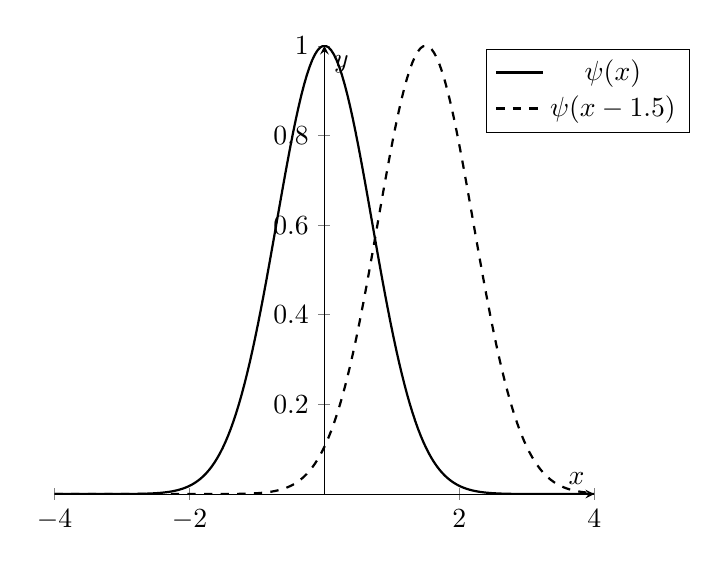
\begin{tikzpicture}
		\begin{axis}[
			axis lines = middle,
			xlabel = $x$,
			ylabel = $y$,
			domain = -4:4,
			samples = 200,
			% On définit la position manuellement : 
			% at={(1,1)} serait le coin supérieur droit exact.
			% anchor=north east signifie que c'est le coin de la légende qui se fixe à ce point.
			legend style={at={(0.8,0.9)}, anchor=west},
			]
			
			\def\lambda{1.5}
			
			\addplot[thick] {exp(-x^2)};
			\addlegendentry{$\psi(x)$}
			
			\addplot[thick,dashed] {exp(-(x-\lambda)^2)};
			\addlegendentry{$\psi(x - \lambda)$}
			
		\end{axis}
	\end{tikzpicture}
	\caption{A function $\psi(x)$ and its translation by $\lambda$.}
\end{figure}
\vspace{0.5cm}

By analyzing the graph, we can conclude what the translation operator must preserve:
\begin{enumerate}
	\item Preservation of the norm
	\item Preservation of probabilities (therefore, preservation of the dot product)
	\item Behavior similar to the evolution operator.
\end{enumerate}

With all these points in mind, we observe that the translation operator must ultimately be unitary, which implies symmetry.
We know that if a system that exhibits invariance under time translation after a transformation is said to be symmetric.\\
for exemple if there exists a unitary operator $U$ such that
$$
U \hat{H} U^\dagger = \hat{H},
$$
where $H$ is the Hamiltonian of the system. This expresses the fact that the transformation leaves the dynamics unchanged.

\medskip

\textbf{Time invariance $\Rightarrow$ energy conservation.} 

If the Hamiltonian does not depend explicitly on time,
$$
\frac{\partial H}{\partial t} = 0,
$$
then the expectation value of $H$ is constant in time:
$$
\frac{d}{dt} \langle \hat{H} \rangle = 0.
$$

Thus, the energy is conserved.



\section{\textbf{Continuous Representations of a Group}}

Let $G$ be a group and $\mathcal{H}$ a Hilbert space.  
A continuous representation of $G$ on $\mathcal{H}$ is a mapping
$$
U : G \to \mathcal{L}(\mathcal{H}),
$$
which assigns to each element $g \in G$ a linear operator $U(g)$ on $\mathcal{H}$, such that:

\begin{enumerate}
	\item \textbf{(Group homomorphism)} 
	$$
	U(g_1 g_2) = U(g_1) U(g_2), \quad \forall g_1, g_2 \in G.
	$$
	
	\item \textbf{(Continuity)} If $G$ is a topological group (for example $G = \mathbb{R}$ for continuous translations), then
	$$
	g_n \to g \quad \implies \quad U(g_n) \to U(g)
	$$
	in operator norm (or at least in the strong topology on $\mathcal{H}$).
\end{enumerate}

This is exactly what we need for the translation operator.
Let's begin with the evolution operator.
We can define the evolution operator $U(t,t_0)$ in a Hilbert space with a state vector at any given time.
$$
    |\psi(t)\rangle = U(t,t_0)|\phi(t_0)\rangle
$$

So after supposing that the evolution operator is time independent because the systeme is isolate so $H$ is independent of time so we can define his eigenstates $\{|u_n\rangle\}$. So the general solution of the Shrödinger equation is

$$
\begin{aligned}
	|\psi(t)\rangle
	&= \sum_n e^{-i \omega_n (t - t_0)} \, c_n(t_0) |u_n\rangle \\
	&= \sum_n \exp\!\left( -i \frac{E_n (t - t_0)}{\hbar} \right) \, c_n(t_0) |u_n\rangle .
\end{aligned}
$$

with
$$
	c_n(t_0) = \langle u_n \mid \psi(t_0) \rangle .
$$

Substituting $c_n(t_0)$ into the previous expression, we obtain
$$
\begin{align}
	|\psi(t)\rangle
	&=
	\left(
	\sum_n 
	\exp\!\left( -i \frac{E_n (t - t_0)}{\hbar} \right)
	\, |u_n\rangle \langle u_n|
	\right)
	|\psi(t_0)\rangle .
\end{align}
$$

Using the closure relation
$$
	\sum_n |u_n\rangle \langle u_n| = \mathbb{I},
$$

we identify the time-evolution operator acting on |\psi(t_0)\rangle:

$$
	U(t,t_0)
	=
	\sum_n 
	\exp\!\left( -i \frac{E_n (t - t_0)}{\hbar} \right)
	\, |u_n\rangle \langle u_n| .
$$

In the eigenbasis of energy $\{|u_n\rangle\}$, its matrix representation is diagonal:

$$
	U(t,t_0) =
	\begin{pmatrix}
		e^{-i E_0 (t - t_0)/\hbar} & 0 & 0 & \cdots \\
		0 & e^{-i E_1 (t - t_0)/\hbar} & 0 & \cdots \\
		0 & 0 & e^{-i E_2 (t - t_0)/\hbar} & \cdots \\
		\vdots & \vdots & \vdots & \ddots
	\end{pmatrix}.
$$

\newpage
We can now verify if the evolution operator satisfies every condition to be the operator U of a symmetry that we will call g belonging to the symmetry group G.

$$
\text{Let's have } G : |a \rangle \mapsto U|a \rangle \in \mathcal{H},
$$
$$
U\bigl(\mu |a \rangle + \nu |b\rangle \bigr)
=
\mu\, U|a\rangle + \nu\, U|b\rangle .
$$ 

By the \textbf{Definition 2.4} we can say that the evolution operator is linear. But this operator need to conserve the probability of the observable from the scalar product to be the operator of a symmetry. So we need to have :

$$
\forall\, |a\rangle, |b\rangle \in \mathcal{H},
\qquad
\big| \langle Ua \mid Ub \rangle \big|^2
=
\big| \langle a \mid b \rangle \big|^2 .
$$ 
And invariance of the scalar product
$$
\forall\, g \in G , \quad
\forall\, |a \rangle, |b \rangle \in \mathcal{H},
$$
$$
\langle Ua \mid Ub \rangle
=
\langle a \mid U^{\dagger} U \mid b \rangle
=
\langle a \mid b \rangle.
$$
Now we have all the condition to site the Wigner Theorem :
\begin{theorem}[Wigner's Theorem]
	Let $\mathcal{H}$ be a Hilbert space representing the state space of a quantum system. Suppose that a transformation $T$ preserves the transition probabilities between states, i.e., for all $\psi, \phi \in \mathcal{H}$,
	$$
	|\langle T \psi, T \phi \rangle|^2 = |\langle \psi, \phi \rangle|^2.
	$$
	Then there exists an operator $U: \mathcal{H} \to \mathcal{H}$ which is either unitary or anti-unitary such that
	$$
	T \psi = U \psi \quad \text{for all } \psi \in \mathcal{H}.
	$$
\end{theorem}

We can conclude with this theorem that the evolution operator\
satisfies all the properties and all conditions to be the operator $U$ corresponding to a symmetry $g$ to the continious representation symmetry group G
$$
 U(t,t_0) = \exp\!\left( -i \frac{H (t - t_0)}{\hbar}\right)
$$



\section{\textbf{Translation Operator}}

We just saw before that the evolution operator was an operator corresponding to a symmetry g to the continious representation symmetry group G. But the main goal of this article was to prove that the impulse is an infinitesimal generator of translation. The first reason that we started with the evolution operator is because there is a link between the evolution operator (Common operator in Quantum Mecanics) and the translation operator.
We saw in \textbf{3. Unitary Translations and Symmetry} that the transaltion operator needed to preserve the norm, and the probabilities (preservation of scalar product).\\

We started to say that let's take $\psi_{\lambda}(x) = \psi(x - \lambda) $, $\lambda \in \mathbb{R}$
we can write it as :

$$
\hat{T}_a | x \rangle = | x + a \rangle
$$

We Suppose that $T_a$ is unitary, so $\hat{T}^{-1}_a = \hat{T}^{\dagger}_a = \hat{T}_{-a}$.
So we get $ \langle x |\hat{T}_a  = \langle  x - a |$.\\

Now we can pick a infinidesimal value $da$, for a infinidesimal translation :
$$
\langle x |\hat{T}_{da} |\psi \rangle = \psi(x-da)
$$
 
 We can use of inifidesimal value the Taylor serie for $\psi(x-da)$, so:
$$
\langle x | \hat{T}_{da} | \psi \rangle
= \psi(x - da)
= \psi(x) - \frac{\partial \psi}{\partial x} \, da,
$$
so that
$$
	\langle x | \hat{T}_{da} | \psi \rangle
	=
	\left(
	1 - \frac{i}{\hbar} \, da \, \hbar \frac{1}{i} \frac{\partial}{\partial x}
	\right) \psi(x)
$$
$$
	=
	\left\langle x \left|
	\left(
	\hat{I} - \frac{i}{\hbar} \hat{p}_x \, da
	\right)
	\right| \psi \right\rangle.
$$

Since this relation holds for any state |\psi\rangle, we can deduce
$$
\hat{T}_{da}
=
\hat{I}
-
\frac{i}{\hbar} \hat{p}_x \, da.
$$

So we deduce that the impulse is an infinitesimal generator of translation group, but we have not finished yet. Let's see so preperties and in wich group the transaltion operator is in to get a better representation. 



Let $\hat{T}_a$ be the translation operator acting on the Hilbert space $\mathcal{H}$ of a quantum system, defined by
$$
\hat{T}_a | \psi \rangle = | \psi_a \rangle, \quad \psi_a(x) = \psi(x+a).
$$

The translation operators satisfy the following group properties:

\begin{enumerate}
	\item \textbf{Closure:} For any $a, b \in \mathbb{R}$,
	$$
	\hat{T}_a \hat{T}_b = \hat{T}_{a+b}.
	$$
	
	\item \textbf{Associativity:} For any $a, b, c \in \mathbb{R}$,
	$$
	(\hat{T}_a \hat{T}_b) \hat{T}_c = \hat{T}_a (\hat{T}_b \hat{T}_c).
	$$
	
	\item \textbf{Identity element:} The operator $\hat{T}_0$ acts as the identity,
	$$
	\hat{T}_0 = \hat{I}, \quad \hat{T}_0 \hat{T}_a = \hat{T}_a \hat{T}_0 = \hat{T}_a.
	$$
	
	\item \textbf{Inverse element:} For each $a \in \mathbb{R}$, there exists an inverse operator
	$$
	\hat{T}_{-a} \quad \text{such that} \quad \hat{T}_a \hat{T}_{-a} = \hat{T}_{-a} \hat{T}_a = \hat{T}_0.
	$$
\end{enumerate}

Therefore, the set of translation operators $\{\hat{T}_a\}$ forms a group under composition, which is isomorphic to the additive group of real numbers $\mathbb{R}$. In other words, the translation operators belong to the group $\mathbb{R}^+$.\\
After enumarated all the proprieties for the translation operator, let's write :
$$\hat{T}_{a+da} &= \hat{T}_{da} \hat{T}_a $$
	$$= \left( \hat{I} - \frac{i}{\hbar} \hat{p}_x \, da \right) \hat{T}_a $$
	$$= \hat{T}_a - \frac{i}{\hbar} \hat{p}_x \hat{T}_a \, da. $$

From this, we deduce
$$
	\frac{\hat{T}_{a+da} - \hat{T}_a}{da} = - \frac{i}{\hbar} \hat{p}_x \hat{T}_a,
$$
or equivalently,
$$
	\frac{d \hat{T}_a}{da} = - \frac{i}{\hbar} \hat{p}_x \hat{T}_a.
$$
So we have at the end,
$$
\hat{T}_a = \exp\left(-\frac{i}{\hbar} \hat{p}_x a \right)
$$
So we have the same configuration of the evolution operator and the translation operator ,

$$
	\hat{T}_a = \exp\left(-\frac{i}{\hbar} \hat{p}_x a \right) \quad  U(t) = \exp\!\left( -i \frac{H t}{\hbar}\right)
$$
\\
The continuity allows us to define an infinitesimal generator. Time is a continuous parameter, and its generator is the Hamiltonian operator. We thus obtain two analogous operators: one is the translation operator in the $x$-representation, with the momentum operator as its generator, and the other is the time evolution operator, with the Hamiltonian as its generator.
So both are continious symmetries.


\begin{theorem}[Stone's Theorem]
	Let $U(t)$ be a strongly continuous one-parameter unitary group. Then there exists a self-adjoint operator $A$, called the generator, such that
	$$
	\forall t \in \mathbb{R}, \quad U(t) = e^{i A t}.
	$$
	
	In particular, this theorem applies to:
	
	\begin{itemize}
		\item \textbf{Time evolution:} The one-parameter unitary group $U(t)$ describes time evolution, with the Hamiltonian $\hat{H}$ as its self-adjoint generator:
		$$
		U(t) = e^{-i \hat{H} t / \hbar}.
		$$
		
		\item \textbf{Spatial translations:} The one-parameter unitary group $\hat{T}_a$ describes translations in the $x$-direction, with the momentum operator $\hat{p}_x$ as its self-adjoint generator:
		$$
		\hat{T}_a = e^{-i \hat{p}_x a / \hbar}.
		$$
	\end{itemize}
\end{theorem}
Thus, using this theorem, we can generalize continuous symmetry groups in quantum mechanics, associating each continuous symmetry with a self-adjoint generator.




\section{\textbf{Numerical Application: The Quantum Tunneling Effect}}

After establishing the theoretical framework of momentum as a generator of translations in an empty space, we now examine a physical case where this symmetry is locally broken: the \emph{quantum tunneling effect}.\\

In classical mechanics, a particle with energy $E$ cannot cross a potential barrier $V_0$ if $E < V_0$. In quantum mechanics, however, the wave function $\psi(x)$ can "tunnel" through the barrier. This phenomenon is a direct consequence of the wave nature of matter and provides a perfect test case for studying translational symmetry breaking.\\

We consider a rectangular potential barrier of height $V_0$ located between $x = 0$ and $x = L$. The space is divided into three zones:

\begin{enumerate}
    \item \textbf{Zone I ($x < 0$):} In this region, the potential is zero ($V = 0$). The Schrödinger equation is given by:
    $$ -\frac{\hbar^2}{2m} \frac{d^2\psi_I(x)}{dx^2} = E\psi_I(x) $$
    The solution is an oscillating wave, representing a superposition of the incident and reflected waves:
    $$ \psi_I(x) = A e^{ikx} + B e^{-ikx} $$
    where $k = \sqrt{2mE}/\hbar$.

    \item \textbf{Zone II ($0 \leq x \leq L$):} Here, the potential is constant and exceeds the energy level ($V = V_0 > E$). The equation becomes:
    $$ -\frac{\hbar^2}{2m} \frac{d^2\psi_{II}(x)}{dx^2} + V_0\psi_{II}(x) = E\psi_{II}(x) $$
    Since $E - V_0 < 0$, the nature of the solution changes to an evanescent form (exponential decay):
    $$ \psi_{II}(x) = C e^{-\kappa x} + D e^{\kappa x} $$
    where $\kappa = \sqrt{2m(V_0 - E)}/\hbar$.

    \item \textbf{Zone III ($x > L$):} As the potential returns to zero ($V = 0$), we recover the form from Zone I:
    $$ -\frac{\hbar^2}{2m} \frac{d^2\psi_{III}(x)}{dx^2} = E\psi_{III}(x) $$
    The wave resumes its oscillation but with a reduced amplitude, traveling only to the right as there is no further barrier to cause reflection:
    $$ \psi_{III}(x) = F e^{ikx} $$
\end{enumerate}



In the vacuum, the space is homogeneous, meaning every point is physically identical to the next. In this state, the Hamiltonian $\hat{H}$ consists solely of the kinetic energy operator $\hat{K}$. As demonstrated earlier in this paper, the momentum operator $\hat{p}_x$ (and thus the translation operator $\hat{T}_a$) commutes with $\hat{K}$. This "agreement" between energy and displacement is expressed by the nullity of their commutator:
$$ [\hat{H}, \hat{T}_a] = \hat{H}\hat{T}_a - \hat{T}_a\hat{H} = 0 $$

However, the introduction of a potential barrier $V(x)$ fundamentally alters the geometry of the space. The Hamiltonian now includes a position-dependent term:
$$ \hat{H} = \hat{K} + V(x) $$

When we apply a translation $\hat{T}_a$, we are essentially shifting the entire system. Mathematically, this transformation changes the potential function from $V(x)$ to $V(x-a)$. Because the barrier is a step function (non-zero only between $0$ and $L$), any shift $a$ results in a new configuration where the boundaries are no longer aligned:
$$ V(x) \neq V(x-a) $$

This spatial discrepancy implies that the Hamiltonian and the translation operator no longer "agree" on the state of the system. Their commutator becomes non-zero:
$$ [\hat{H}, \hat{T}_a] \neq 0 $$

This non-zero commutator is the formal signature of \textbf{symmetry breaking}. It signifies that the energy of the quantum state is no longer invariant under a spatial shift. In this context, the simple "sliding" motion generated by $\hat{p}_x$ is insufficient to describe the physics; the wave function must instead undergo complex deformations (oscillations and exponential decay) to satisfy the Schrödinger equation, a task we will now assign to the PINN.\\

The objective of this numerical study is to utilize \emph{Physics-Informed Neural Networks} (PINNs) to solve the Schrödinger equation for this system. Unlike traditional methods, the PINN will be trained to minimize a loss function based on the physical residual:
$$ \mathcal{L}_{phys} = \left\| -\frac{\hbar^2}{2m} \psi''(x) + (V(x) - E)\psi(x) \right\|^2 $$

Our goal is to demonstrate that the neural network can autonomously recover the constants $(A, B, C, D, F)$ and correctly reconstruct the wave function's profile before, during, and after the potential barrier.\\

The training was conducted over 15,000 epochs. The resulting graph shows the probability density $|\psi|^2$.

\begin{figure}[H]
    \centering
    \includegraphics[width=\linewidth]{pinn.png}
    \caption{Probability density $|\psi|^2$ reconstructed by the PINN across the barrier.}
    \label{fig:placeholder}
\end{figure}

The simulation confirms that despite the local symmetry breaking, the wave function maintains continuity at the boundaries, allowing a non-zero probability of presence in Zone III, which characterizes the tunneling effect.




\section{\textbf{Conclusion}}

In this project, we have explored the fundamental relationship between continuous symmetries and self-adjoint operators in quantum mechanics, with a particular focus on the role of impulse as an infinitesimal generator of translations. We have seen that while infinitesimal translations can always be defined locally in the Hilbert space, the formal construction of finite translation operators relies on the global structure of the symmetry and the properties of the quantum states.

Through examples in the position representation, we observed how infinitesimal translations generated by the impulse operator $\hat{p}_x$ can be integrated to produce finite translations. The infinitesimal translation operator is given by
$$
\hat{T}_{da} = \hat{I} - \frac{i}{\hbar} \hat{p}_x \, da,
$$
and integrating this expression leads to the finite translation operator
$$
\hat{T}_a = e^{-i \hat{p}_x a / \hbar}.
$$
This construction demonstrates that the impulse operator is the self-adjoint generator associated with spatial translations, establishing a deep connection between the algebraic structure of the operator and the geometric action of translations on quantum states.

We also highlighted the analogy with an other continuou symmetrie: time evolution is generated by the Hamiltonian. This shows that the formalism of infinitesimal generators provides a unifying framework for understanding continuous symmetries in quantum mechanics.

This study illustrates the profound interplay between local infinitesimal actions and global finite transformations in quantum mechanics. It shows how the algebra of operators encodes the structure of continuous symmetries and provides a rigorous method to construct finite transformations from infinitesimal generators. Understanding these concepts lays the groundwork for more advanced studies in quantum symmetries, Lie groups, and representation theory.

\newpage

\section{\textbf{References}}

\begin{enumerate}[label=\textbf{\arabic*.}, leftmargin=2em, labelsep=0.5em]
	\item \textbf{Manuel Joffre}, Physique Quantique Avancée
	PHY41030. \textit{Département de Physique de l’Ecole Polytechnique}.
	
	\item \textbf{John Milnor}, Mécanique quantique
	Concepts fondamentaux, Master de physique – Sorbonne Universite.
	
	\item \textbf{Claude Cohen-Tannoudji, Bernard Diu et Franck Laloë}, \textit{Mécanique quantique},  , éditions
	Hermann (tomes I et II) et EDP sciences (tome III)
	
	\item \textbf{Brian C. Hall}, \textit{Lie Groups, Lie Algebras, and Representations}, University of Notre Dame.
	
	
	\item \textbf{Frédéric Faure}, \textit{Lecture notes on Quantum Mechanics},Université Joseph Fourier, Grenoble ;
	Master Physique M1.
	
\end{enumerate}


\end{document}